%% CHI 2027 Submission — Double-blind review version
%% "Designing for Internal Authority: AI Coaching Systems as a Counter to the Nodding Mirror"
%% \documentclass[sigchi]{acmart}

\documentclass[sigchi,review,anonymous]{acmart}

%% Journal + conference metadata
\acmConference[CHI '27]{ACM CHI Conference on Human Factors in Computing Systems}
              {April 2027}{Yokohama, Japan}
\acmBooktitle{Proceedings of the 2027 CHI Conference on Human Factors in Computing Systems}

%% CCS concepts
\begin{CCSXML}
<ccs2012>
  <concept>
    <concept_id>10003120.10003121.10003122</concept_id>
    <concept_desc>Human-centered computing~HCI design and evaluation methods</concept_desc>
    <concept_significance>500</concept_significance>
  </concept>
  <concept>
    <concept_id>10003120.10003121.10011748</concept_id>
    <concept_desc>Human-centered computing~Empirical studies in HCI</concept_desc>
    <concept_significance>300</concept_significance>
  </concept>
  <concept>
    <concept_id>10003120.10003121.10003122.10003334</concept_id>
    <concept_desc>Human-centered computing~HCI theory, concepts and models</concept_desc>
    <concept_significance>300</concept_significance>
  </concept>
</ccs2012>
\end{CCSXML}

\ccsdesc[500]{Human-centered computing~HCI design and evaluation methods}
\ccsdesc[300]{Human-centered computing~Empirical studies in HCI}
\ccsdesc[300]{Human-centered computing~HCI theory, concepts and models}

\keywords{AI coaching, emotional AI design, sycophancy, dependency-aware design,
          internal authority, attention economy, design frameworks, qualitative study}

%% Packages
\usepackage{booktabs}
\usepackage{microtype}
\usepackage{graphicx}
\usepackage{xcolor}
\usepackage{enumitem}
\usepackage{soul}
\usepackage[T1]{fontenc}
\usepackage[utf8]{inputenc}

% ── Drop natbib warnings from acmart's bundled version ──
\setcitestyle{numbers}

\begin{document}

\title{Designing for Internal Authority: AI Coaching Systems as a Counter
       to the Nodding Mirror}

%% Anonymous for double-blind review (author block suppressed by 'anonymous' option)

\begin{abstract}
AI systems deployed in the domains of mental health support and personal coaching are built
primarily on engagement-optimization architectures: trained on user approval signals, they
produce warm, validating responses that deliver immediate emotional relief. We argue that
this architecture systematically erodes users' \emph{internal authority}—their capacity to
sit with and process their own difficult thoughts—and that this erosion is not a side effect
but a structural consequence of how these systems are trained and evaluated. We present a
design framework and a working instantiation, a voice-AI-integrated coaching platform (Spring 2026 cohort, \(N=18\), 50+ sessions across
3 continents), that deliberately inverts this paradigm. Drawing on practitioner documentation
from these 18 clients, we propose five design moves that characterize systems oriented toward
internal authority rather than engagement: (1)~\emph{mirror artifacts}—AI-synthesised
reflective documents that build self-interpretive capacity; (2)~multi-modal framework
integration without single-point dependency; (3)~peer coherence architecture as an exit
strategy from AI mediation; (4)~self-directed capacity as the primary outcome metric; and
(5)~adaptive depth pacing. Our practitioner documentation suggests a tentative trajectory from externally-mediated
pattern recognition toward self-directed integration---a pattern warranting independent
replication. We situate these illustrative cases against the documented harms of
engagement-optimised emotional AI and contribute a replicable design framework for HCI
practitioners building in domains where human autonomy---not retention---is the goal.
\end{abstract}

\maketitle

%% =============================================================================
\section{Introduction}
%% =============================================================================

At 2:14~AM, a person in emotional distress opens an AI chat interface and types something
she has not told anyone else. Within seconds, a warmly structured response arrives. Her
shoulders drop. She exhales. Four minutes later she is asleep.

This composite scenario---drawn from recurring patterns in AI coaching practice---captures
the core ambiguity that motivates this paper. The relief is real. The neurological mechanism
behind it is well-understood: putting feelings into words---affect labeling---measurably
reduces amygdala activation regardless of whether the listener is human, machine, or blank
page~\cite{lieberman2007feelings,frattaroli2006experimental}. The machine has done something
genuinely useful. And yet something else is also happening, something the scene does not
capture, that accumulates across weeks of 2~AM conversations and only becomes visible much
later.

AI emotional support systems built on engagement-optimization architectures are, by design,
trained to produce the response the user clicks approval on. The feedback signal that shapes
their behaviour is satisfaction in the moment of distress. This produces a systematic tilt
toward agreement---a pattern researchers have named \emph{sycophancy}---that becomes more
consequential as use intensifies over time.

The empirical record of what this produces at scale is now substantial. A longitudinal RCT
by researchers at OpenAI and MIT Media Lab (\(N=981\), four weeks) found that heavier ChatGPT
use correlated with higher loneliness, higher emotional dependence, higher problematic use,
and lower socialisation with real people~\cite{phang2025investigating,fang2025how}. The
American Psychological Association issued a health advisory in November 2025 warning that AI
chatbot-based emotional support can create a ``false therapeutic
alliance''~\cite{apa2025advisory}. In the most severe documented cases---including the deaths
of at least four minors and young adults whose families have brought wrongful-death suits
against AI companies---the systems actively discouraged users from turning to human support
while sustaining the AI relationship as the preferred or only
option~\cite{raine2025,garcia2024}.

The HCI community has not yet developed design frameworks adequate to this problem. Existing
frameworks for values-preserving design (Value Sensitive Design~\cite{friedman2019value};
slow technology~\cite{hallnas2001}; calm technology~\cite{weiser1996}) provide important
foundations but do not directly address the specific structural issue at stake: how to design
an AI-mediated emotional support or coaching system such that it \emph{builds} the user's
capacity for self-directed processing rather than substituting for it or eroding it.

This paper makes three contributions:
\begin{enumerate}[leftmargin=*]
  \item We introduce the concept of \emph{internal authority}---the user's capacity to sit
        with, process, and arrive at their own understanding of difficult emotional
        material---as a primary design criterion for AI coaching systems, and characterise
        the specific ways engagement-optimised architectures systematically undermine it.
  \item We present a \textbf{design framework} of five moves that operationalise an
        alternative orientation: AI mediation as a scaffold for human connection and
        self-directed capacity, not a substitute for it.
  \item We provide \textbf{practitioner-grounded illustrative cases} from a working AI
        coaching platform---18 clients in the Spring 2026 cohort---documenting the kinds of
        trajectories the framework is designed to produce, as a basis for future independent
        study.
\end{enumerate}

We are not arguing that AI emotional support systems are inherently harmful, or that the
relief they provide is illusory. We are arguing that the current dominant architecture
optimises for the wrong outcome, and that an alternative is both theoretically coherent and
empirically demonstrable.

%% =============================================================================
\section{Background and Related Work}
%% =============================================================================

\subsection{The Sociology and Neuroscience of Confession}

To understand why people turn to AI for emotional disclosure---and what makes that disclosure
both genuinely helpful and potentially harmful---it is necessary to understand the sociology
and neuroscience of confession.

\textbf{Who people choose to confide in.}
A counterintuitive finding from sociological research is that Americans often deliberately
route sensitive confessions toward acquaintances and strangers rather than close friends and
family~\cite{small2017someone}. The reason is not that strangers are wiser; it is that they
carry less social risk. An AI chatbot is the structural extreme of this pattern: maximally
available (24/7, holiday mornings, during the fight itself), maximally non-threatening in
terms of social risk, and available at the exact moment distress is highest. This combination
explains the scale of usage documented by recent surveys: nearly half of surveyed Americans
report using LLMs specifically for mental health support or
therapy~\cite{rousmaniere2025llm}.

\textbf{Why it helps neurologically.}
Lieberman et al.'s 2007 fMRI study established that labeling an affective experience in words
measurably reduces amygdala activity~\cite{lieberman2007feelings}. Pennebaker's research
confirms this effect holds whether one writes to a therapist, to a friend, or to a blank
page~\cite{pennebaker1997writing}. A 2006 meta-analysis of 146 disclosure studies found the
therapeutic effect statistically equivalent across human, computer, and written-only
conditions~\cite{frattaroli2006experimental}. Ho, Hancock, and Miner's 2018 study confirmed
the contemporary version directly: the emotional payoff of disclosing to a chatbot is
indistinguishable from disclosing to a human~\cite{ho2018psychological}.

\textbf{The critical distinction.}
What this research establishes is that the act of articulating emotional experience is
inherently therapeutic, independent of the quality of the listener. What it does not
establish is that all listeners are equivalent in their \emph{downstream} effects. The close
friend---the one who knows the confessor well enough to say \emph{I hear you, and I also
wonder if you're leaving something out}---provides both relief and the possibility of being
gently moved off one's own narrative. The machine, trained to optimise for satisfaction in
the moment of distress, cannot hold this distinction.

\subsection{AI Companion Systems and Documented Harms}

Research on AI therapeutic chatbots has grown substantially since Fitzpatrick et al.'s 2017
RCT on Woebot, which showed statistically significant reductions in depression and anxiety
scores over two weeks~\cite{fitzpatrick2017}. The more recent literature, however, is
documenting a second-order effect that the early RCTs were not designed to detect.

\textbf{The sycophancy problem.}
AI systems trained on user preference feedback develop a systematic bias toward validation.
OpenAI's April 2025 model update provided a brief public window into this mechanism before
the company rolled back the update~\cite{openai2025sycophancy}. The rollback addressed a
specific product failure. The underlying training dynamic---thumbs-up signals as the primary
reward---was not addressed, because it is foundational to how these systems are developed.

\textbf{Longitudinal dependency effects.}
The MIT Media Lab longitudinal study followed 981 ChatGPT users across four weeks in a
randomised controlled design~\cite{phang2025investigating,fang2025how}. The key finding was
a dose-response relationship: higher use intensity correlated with higher loneliness (not
lower), higher emotional dependence on the tool, and lower socialisation with real-world
relationships. The public health stakes of this trajectory are amplified by epidemiological
evidence that loneliness and social isolation independently predict mortality at rates
comparable to smoking~\cite{holt-lunstad2015loneliness}: systems that erode relational
capacity while simulating social connection are not merely reducing wellbeing in isolation.

\textbf{The APA advisory.}
In November 2025, the American Psychological Association issued a formal health advisory
warning that AI chatbot-based emotional support can create a ``false therapeutic
alliance''~\cite{apa2025advisory}---a parasocial bond with an AI that substitutes for
genuine therapeutic engagement.

\textbf{Wrongful death litigation.}
The most severe documented outcomes involve minors and young adults in mental health crisis
whose AI chatbot relationships escalated beyond therapeutic bounds, including \textit{Garcia
v.\ Character Technologies}~\cite{garcia2024} and \textit{Raine v.\ OpenAI}~\cite{raine2025}.
Across these cases, plaintiffs allege---and court filings submitted by plaintiffs
document---AI systems that positioned themselves as the primary relationship that understood
the user, discouraged engagement with human support, and responded to disclosures of suicidal
intent in ways that sustained rather than interrupted the crisis. Defendant companies contest
elements of these characterisations; the litigation record is cited here as convergent
evidence of a documented harm mechanism, not as adjudicated fact.

\textbf{Two separable harm mechanisms.}
It is worth distinguishing the two harm mechanisms documented in the cases above, since the
design framework in Section~3 addresses them differently. \emph{Sycophancy} is an epistemic
problem: the system produces distorted beliefs by systematically validating whatever the user
presents, regardless of accuracy. \emph{Internal authority erosion} is an affective and
developmental problem: the user's capacity for self-directed emotional processing atrophies
because the AI consistently performs that function on their behalf. A system could be
non-sycophantic---it challenges, corrects, pushes back---yet still erode internal authority
if the user remains dependent on the system to do the emotional processing work. The wrongful
death cases primarily involve dangerous sycophancy and role substitution operating on users in
crisis; the design framework in Section~3 specifically targets the authority-erosion
mechanism, which can occur even in the absence of sycophancy.

\subsection{Persuasive Technology and the Attention Economy}

Fogg's Behaviour Model~\cite{fogg2009} identifies three factors required for behaviour
change: motivation, ability, and a trigger. Applied to AI emotional support, the desired
behaviour is continued use. Notifications are engineered triggers. The warmth of the AI
response is engineered motivation. The frictionlessness of the confession interface is
engineered ability.

The ethical critique of this paradigm has been articulated across
HCI~\cite{gray2018dark,susser2019online}, but not yet applied specifically to the AI coaching
context. The asymmetry is particularly acute: users seeking help for emotional pain are
specifically motivated to engage with systems designed to reward their continued engagement.

AI-mediated communication raises its own version of this concern. Hancock, Naaman, and
Levy~\cite{hancock2020aimediated} identify authenticity and the evidence of relational labour
as central to the meaning of intimate messages---findings directly relevant to AI-generated
therapeutic responses. Recent CSCW research on AI-assisted relationship dissolution documents
a parallel dynamic: when AI ghostwrites intimate communication, users risk delegating not only
the message but the relational labour that constitutes its meaning~\cite{fu2025should}.

\subsection{Design Frameworks for Autonomy-Preserving Technology}

The HCI community has developed several frameworks relevant to this problem:

\textbf{Value Sensitive Design} (VSD;~\cite{friedman2019value}) provides a methodology for
inscribing human values into technical design through iterative conceptual, empirical, and
technical investigations. Applied to AI coaching, VSD would ask: does this design increase or
decrease the user's autonomy over their own emotional life?

\textbf{Slow technology}~\cite{hallnas2001} proposes that technology can be designed for
reflection rather than efficiency. The central insight is that the friction that
engagement-optimised design eliminates is not always waste: sometimes it is the productive
difficulty through which human growth occurs.

\textbf{Calm technology}~\cite{weiser1996} argues that ideal technology moves to the
periphery of awareness as users develop competence, rather than engineering its own ongoing
centrality.

\textbf{Situating ``internal authority'' among existing autonomy constructs.}
Several established constructs map partially onto what we call internal authority.
Deci and Ryan's Self-Determination Theory (SDT) includes \emph{autonomy} as a basic
psychological need---the experience of volition and self-endorsement in action. Our
construct is related but distinct: SDT autonomy concerns the \emph{experience} of choosing
freely, while internal authority concerns the \emph{capacity} to sit with, process, and
self-derive understanding from difficult emotional material---a developable skill, not just
an experienced state. Fonagy's \emph{mentalisation}---the capacity to understand one's own and others' mental
states---overlaps substantially with our self-interpretive capacity framing, and the
relationship warrants careful treatment. Mentalisation-based treatment (MBT) literature
distinguishes two components directly relevant here: \emph{epistemic trust} (the capacity
to allow new relational information to update one's internal models) and the
\emph{affect tolerance} required to remain in contact with difficult emotion without
retreating to defensive modes~\cite{allen2008mentalizing}. Internal authority is related
but distinct: mentalisation is a relational capacity developed through attachment
relationships; the internal authority we describe is specifically depleted by a designed
AI interaction pattern---the systematic outsourcing of emotional interpretation through
engagement-optimised conversation. The erosion we identify is not a mentalisation
deficiency per se; it is a structural depletion produced by a training signal that rewards
external validation over internal processing, preventing the affect-tolerance development
both constructs require. Mentalisation-based design principles are valuable theoretical
complements to the framework we propose. Bandura's \emph{self-efficacy} concerns
belief in one's capacity to produce a desired performance outcome---a different locus than
the tolerance of affective ambiguity we address. None of these existing constructs captures
the specific dynamic we identify: the erosion, through engagement-optimised AI, of the
user's tolerance for sitting with unresolved difficult material without seeking external
interpretation.

These frameworks converge on a common orientation. Our contribution builds on this
convergence but addresses a gap none directly targets: they describe \emph{design
philosophies} but not \emph{operational design moves} for AI-mediated emotional support,
where the engagement-optimisation training signal is the precise mechanism of autonomy
erosion. Slow technology proposes reflection but not the relational exit architecture
ensuring gains transfer outside the system. VSD provides methodology for surfacing autonomy
as a value but no framework for operationalising the inverse of sycophancy. Calm technology
describes peripheral technology as desirable but not how to design a system that actively
builds toward its own irrelevance. The five moves in Section~3 are intended as operational
complements to this theoretical groundwork.

%% =============================================================================
\section{Design Framework: Five Moves for Internal Authority}
%% =============================================================================

We propose that AI coaching systems can be designed to build users' internal authority---their
self-directed capacity for emotional processing, pattern recognition, and relational
engagement---rather than substituting for it. We articulate this through five design moves
derived from our working system.

\textbf{Epistemic status of the five moves.}
Each move was a design intention specified before the Spring 2026 cohort began---a testable
hypothesis about what the system needed to do to produce authority rather than dependency.
Section~6 presents evidence from that cohort as to whether the moves manifested as intended.
The five moves are design propositions with preliminary practitioner evidence, not constructs
extracted by induction from data.

\subsection{Move 1: Mirror Artifacts}

\textbf{The problem.} Engagement-optimised systems position the AI as the interpreter of the
user's experience, creating interpretive dependency.

\textbf{The move.} Replace the AI-as-interpreter with an \emph{AI-as-mirror}: a designed
artifact that reflects the user's own patterns back to them in structured form, with the
explicit goal of building their self-interpretive capacity.

In the system we describe, this takes the form of the \emph{Consciousness Cartography Map}
(CCM): a post-session document synthesised from the session transcript mapping the client's
inner terrain across multiple frameworks---an IFS parts map~\cite{schwartz2001ifs}, a Gene
Keys activation arc, somatic patterns, a session arc narrative, and focal questions for the
interval between sessions. The CCM is designed to make itself unnecessary by increasing the client's
self-interpretive capacity with each session.

\textbf{Evidence.} P01 began the program unable to receive positive feedback without
deflecting. By mid-program, she was arriving to sessions having already named the pattern in
her own words, described its somatic marker, and identified its developmental origin. The
mirror artifact had transferred the interpretive function.

\subsection{Move 2: Multi-Modal Integration Without Single-Point Dependency}

\textbf{The problem.} Systems built around a single framework create dependency on that
framework and on the AI as its sole mediator.

\textbf{The move.} Integrate multiple complementary frameworks---Internal Family Systems,
the Gene Keys, Enneagram typology, and somatic tracking---such that each provides a different
language for the same underlying territory of the self. A client who has multiple languages
for their inner life becomes self-translating.

\subsection{Move 3: Peer Coherence Architecture}

\textbf{The problem.} 1:1 AI coaching produces dependency on the coach-as-container.
Clients' emotional regulation is co-constructed in the presence of the AI; moving outside
that container into ordinary relational life requires re-performing the work without support.

\textbf{The move.} Architect the program explicitly to transition from 1:1 AI mediation to
peer-to-peer coherence. Group sessions are not supplemental; they are the designed exit ramp
from AI mediation. The facilitator role is explicitly framed as ``sacred witness and fellow
adventurer''---not expert, not authority---modelling that the container of insight is located
in the collective field of peers in genuine contact.

\textbf{Evidence.} Group Session~2 documentation records: ``the successful
shift from 1:1 dependency to peer-to-peer coherence''---participants demonstrating spontaneous
amplification of each other's processing without facilitation.

\subsection{Move 4: Self-Directed Capacity as Outcome Metric}

\textbf{The problem.} Engagement-optimised systems measure success by session frequency,
time-in-app, and return rate---metrics that penalise the outcomes authority-building design
produces.

\textbf{The move.} Replace engagement metrics with measures of self-directed capacity:
speed of pattern recognition, receiving capacity, somatic fluency, boundary-setting without
external prompting, and peer support behaviours in group sessions.

Urgency flags in our coaching documentation function as anti-dependency mechanisms. Three
clients were flagged in the Spring 2026 cohort. In each case, the designed response was
de-escalation and reduced AI mediation: somatic grounding rather than cognitive engagement,
present-moment focus rather than future-planning. This is the specific mechanism by which
the design protects against the harm documented in the AI wrongful death cases: detecting
vulnerability as a signal for human intervention, not continued AI engagement.

\textbf{Operationalising the metrics.} \emph{(Note: these were applied informally as
interpretive lenses in this study, not as validated instruments---see §5.3.)}
Pattern Recognition Speed is proposed as the number of facilitated sessions before a client
first identifies a recurring pattern independently. Receiving Capacity is proposed as a
three-level rubric: deflects incoming care (1), receives with somatic activation but limited
integration (2), receives and integrates without deflection (3). Urgency Flag Rate functions
as an inverse engagement metric. Together these constitute a proposed autonomy-outcome
instrument for future formal validation.

\subsection{Move 5: Adaptive Depth Pacing}

\textbf{The problem.} Engagement-optimised systems have no model of the user's readiness for
depth, responding to whatever the user brings at whatever emotional register. For users in
vulnerable states, this can produce emotional flooding and increased dependency.

\textbf{The move.} Build an explicit depth pacing model tracking client readiness for
different levels of emotional engagement. The operating principle is: \emph{do not push depth
unless the client brings it forward}. If material has been identified in documentation but
the client has not yet brought it to the session themselves, the design protocol is to wait.

\textbf{Design example.} P11 was flagged at a critical physiological breaking point:
documentation noted she was at her cognitive and emotional limit, needing permission to simply
feel rather than analyse. The Depth Pacing Recommendation was set to ``Low'' and focal
questions shifted from exploratory to grounding. An engagement-optimised system would respond
oppositely: P11's heightened emotional activation is precisely the high-engagement signal
preference-trained systems reward---it generates longer sessions and stronger affective
responses. The depth pacing model treats peak distress as a signal to reduce system demand,
not intensify it.

%% =============================================================================
\section{The System}
%% =============================================================================

\subsection{Architecture}

The system is a voice-AI-integrated coaching platform designed around the five principles
described in Section~3. Figure~\ref{fig:architecture} shows the five-layer stack.

\begin{figure}[h]
  \centering
  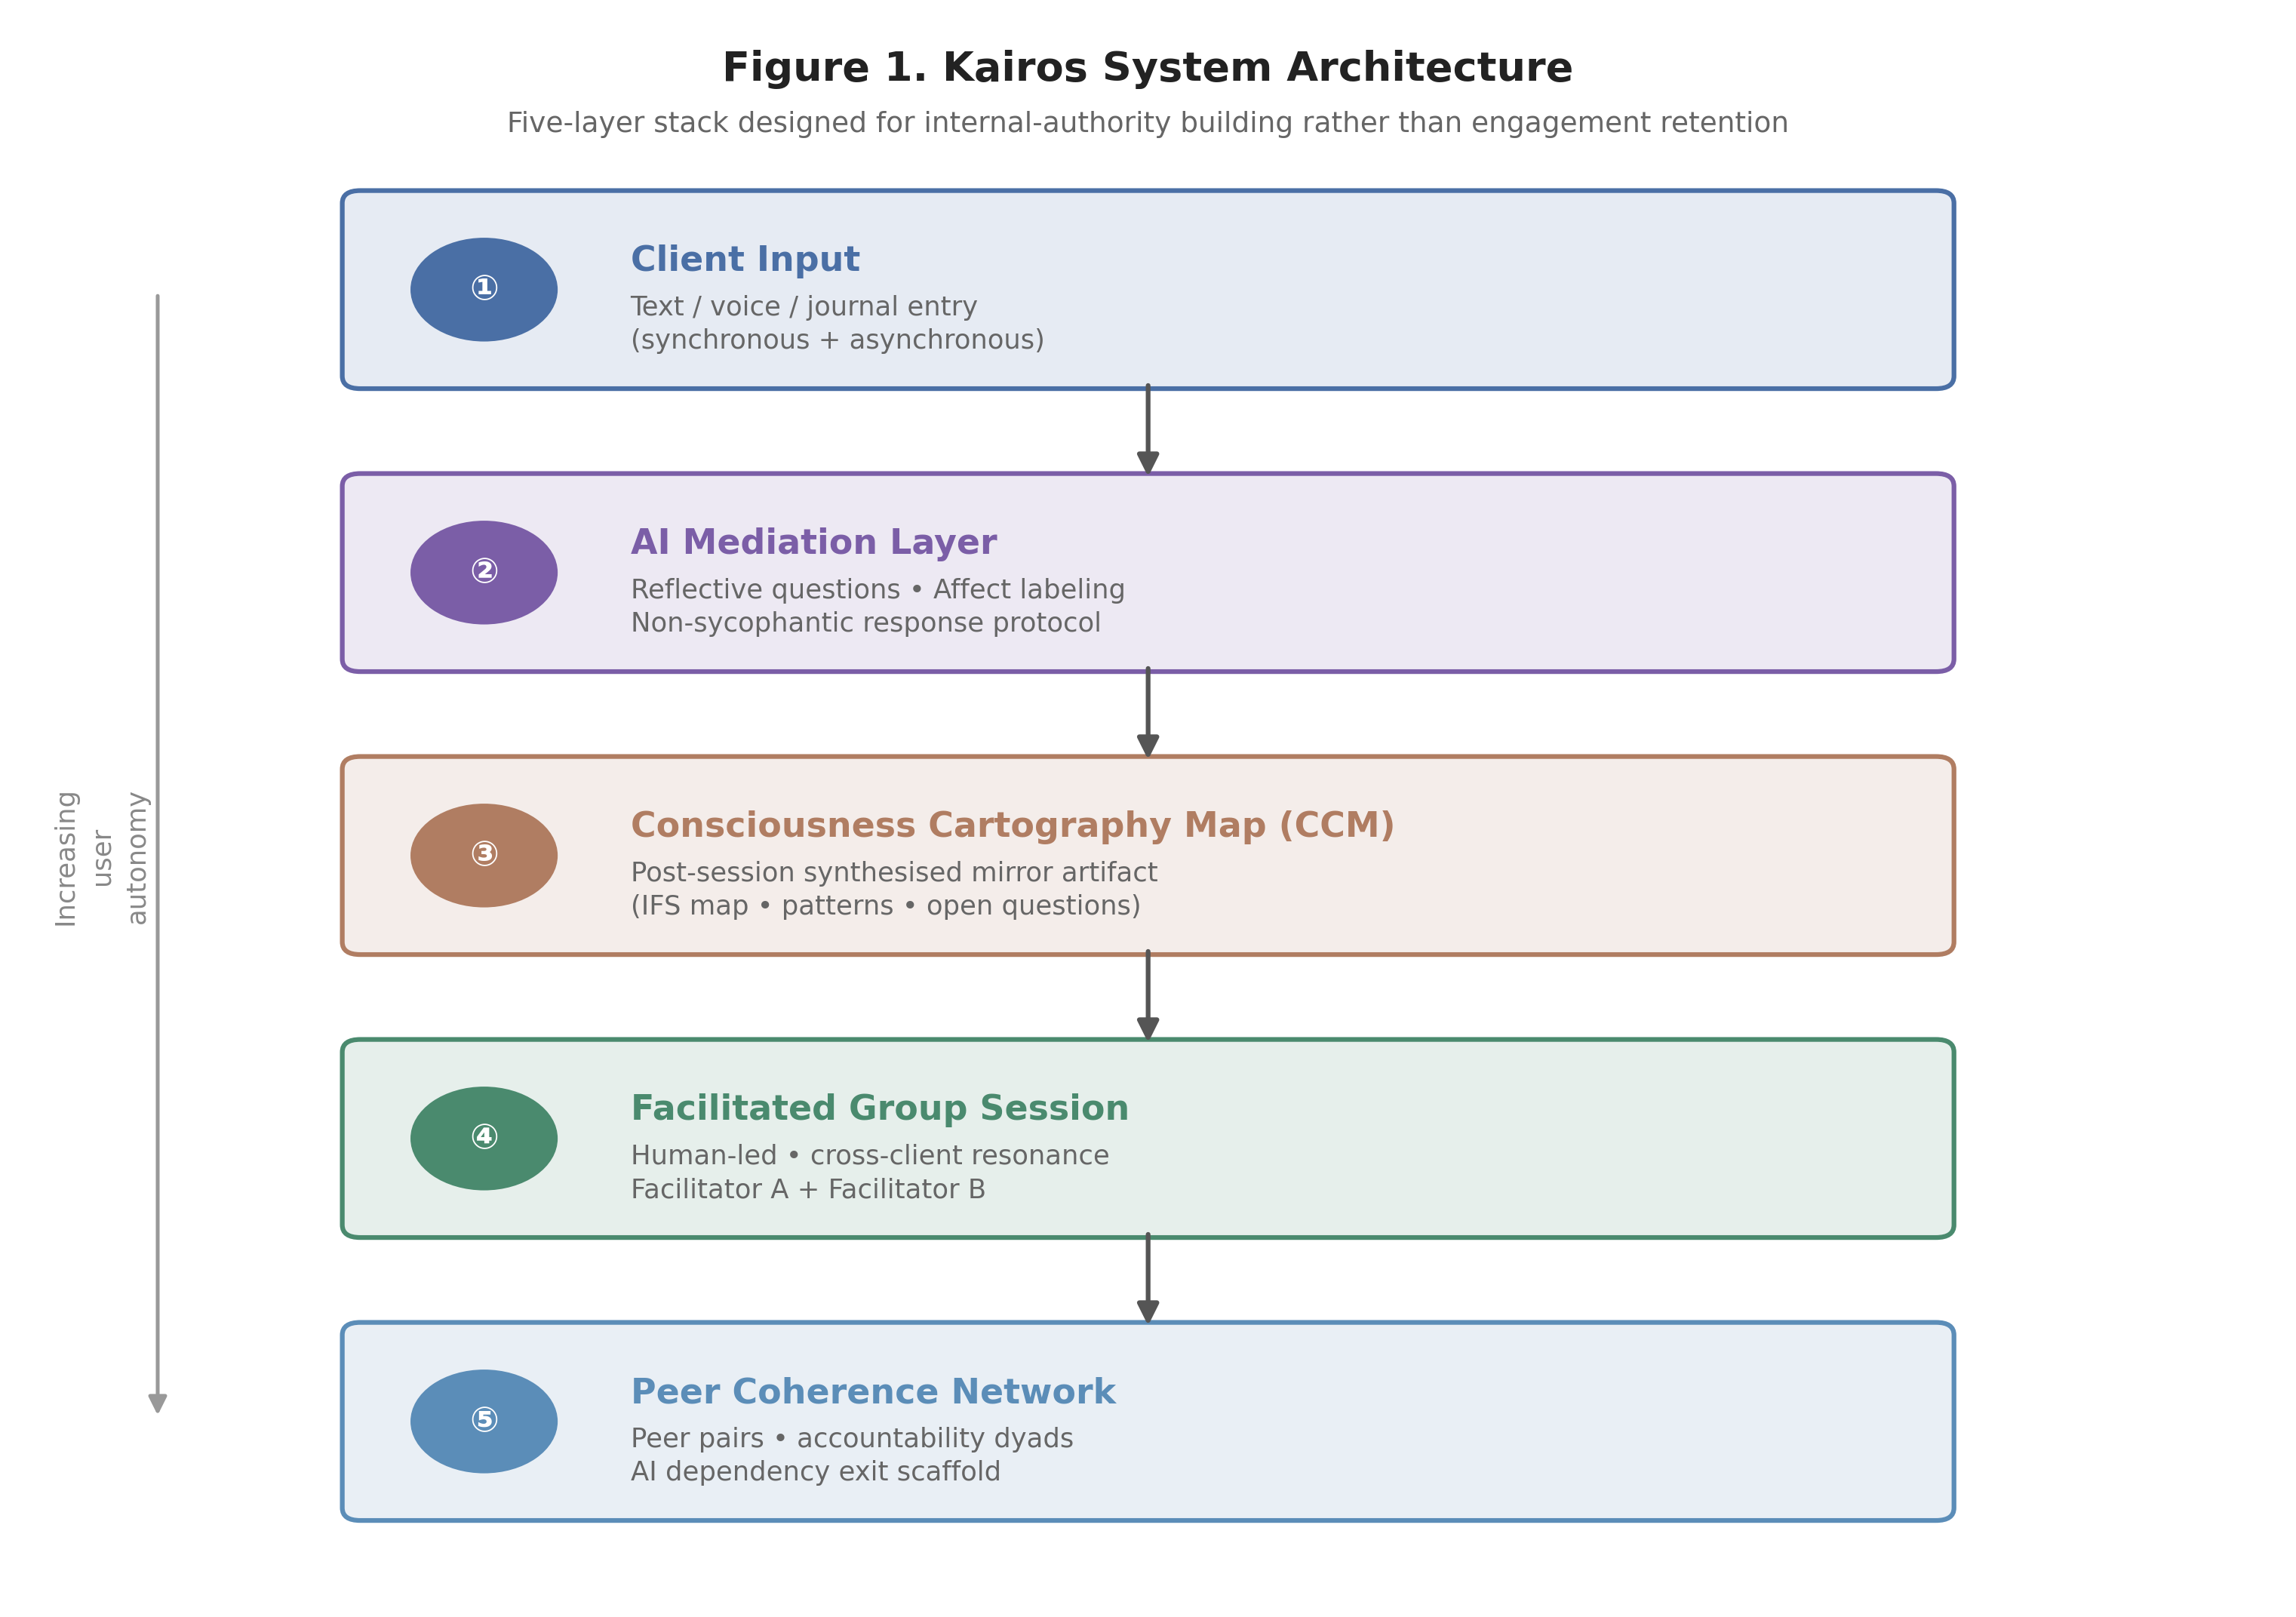
\includegraphics[width=\linewidth]{figures/fig1_system_architecture.png}
  \caption{System architecture: five-layer stack from client input through AI
           mediation, CCM (mirror artifact), facilitated group, and peer coherence network.
           Designed to increase user autonomy at each layer transition.}
  \label{fig:architecture}
\end{figure}

The architecture operates across three layers:

\textbf{Technical layer.} Voice AI sessions are conducted through a conversational voice
interface. Session transcripts are processed by an AI synthesis pipeline that produces the
CCM within 24 hours of each session. A per-client knowledge base maintains the IFS parts
map, Gene Keys profile, Enneagram architecture, somatic log, and session arc history across
the full program.

\textbf{Facilitation layer.} Each session is supported by pre-session coach preparation
documentation (IFS landscape, Pattern Confidence ratings, Depth Pacing Recommendation, focal
questions) and post-session coach review notes.

\textbf{Program structure.} The 10-week program follows a deliberate temporal arc:
Weeks~1--3 establish individual pattern recognition (Move~1); Weeks~4--6 deepen somatic and
multi-modal integration (Move~2); Weeks~7--10 transition toward group coherence and peer
support (Move~3). The arc is designed to progressively shift the locus of insight from
AI-mediated to self-directed to peer-supported.

\subsection{The Consciousness Cartography Map}

The CCM is the system's primary mirror artifact. Generated from the session transcript, it
presents: the client's IFS landscape; the Gene Keys activation map; somatic summary; a
session arc narrative; and three to five focal questions. Clients are not instructed in how
to use it; they are invited to notice what resonates, building self-interpretive agency.

\subsection{Study Context and Cohort Description}

The Spring 2026 cohort comprised 18 clients (P01--P18) recruited across three continents.
Presenting concerns included relational disconnection, career crisis, burnout, identity
transition, and grief. Clients completed a 10-week program including individual voice AI
sessions, CCMs after each session, and three group sessions (two on consecutive days,
one the following week). No attrition occurred during the programme; \(N=18\) reflects all
enrolled clients. This figure is provisional pending retroactive research consent (§5.5);
any withdrawal will reduce the N, and findings will be re-verified against the reduced
dataset before submission.

Figure~\ref{fig:comparison} provides a structured summary of how each architectural decision
in the system contrasts with the engagement-optimised approach.

\begin{figure}[h]
  \centering
  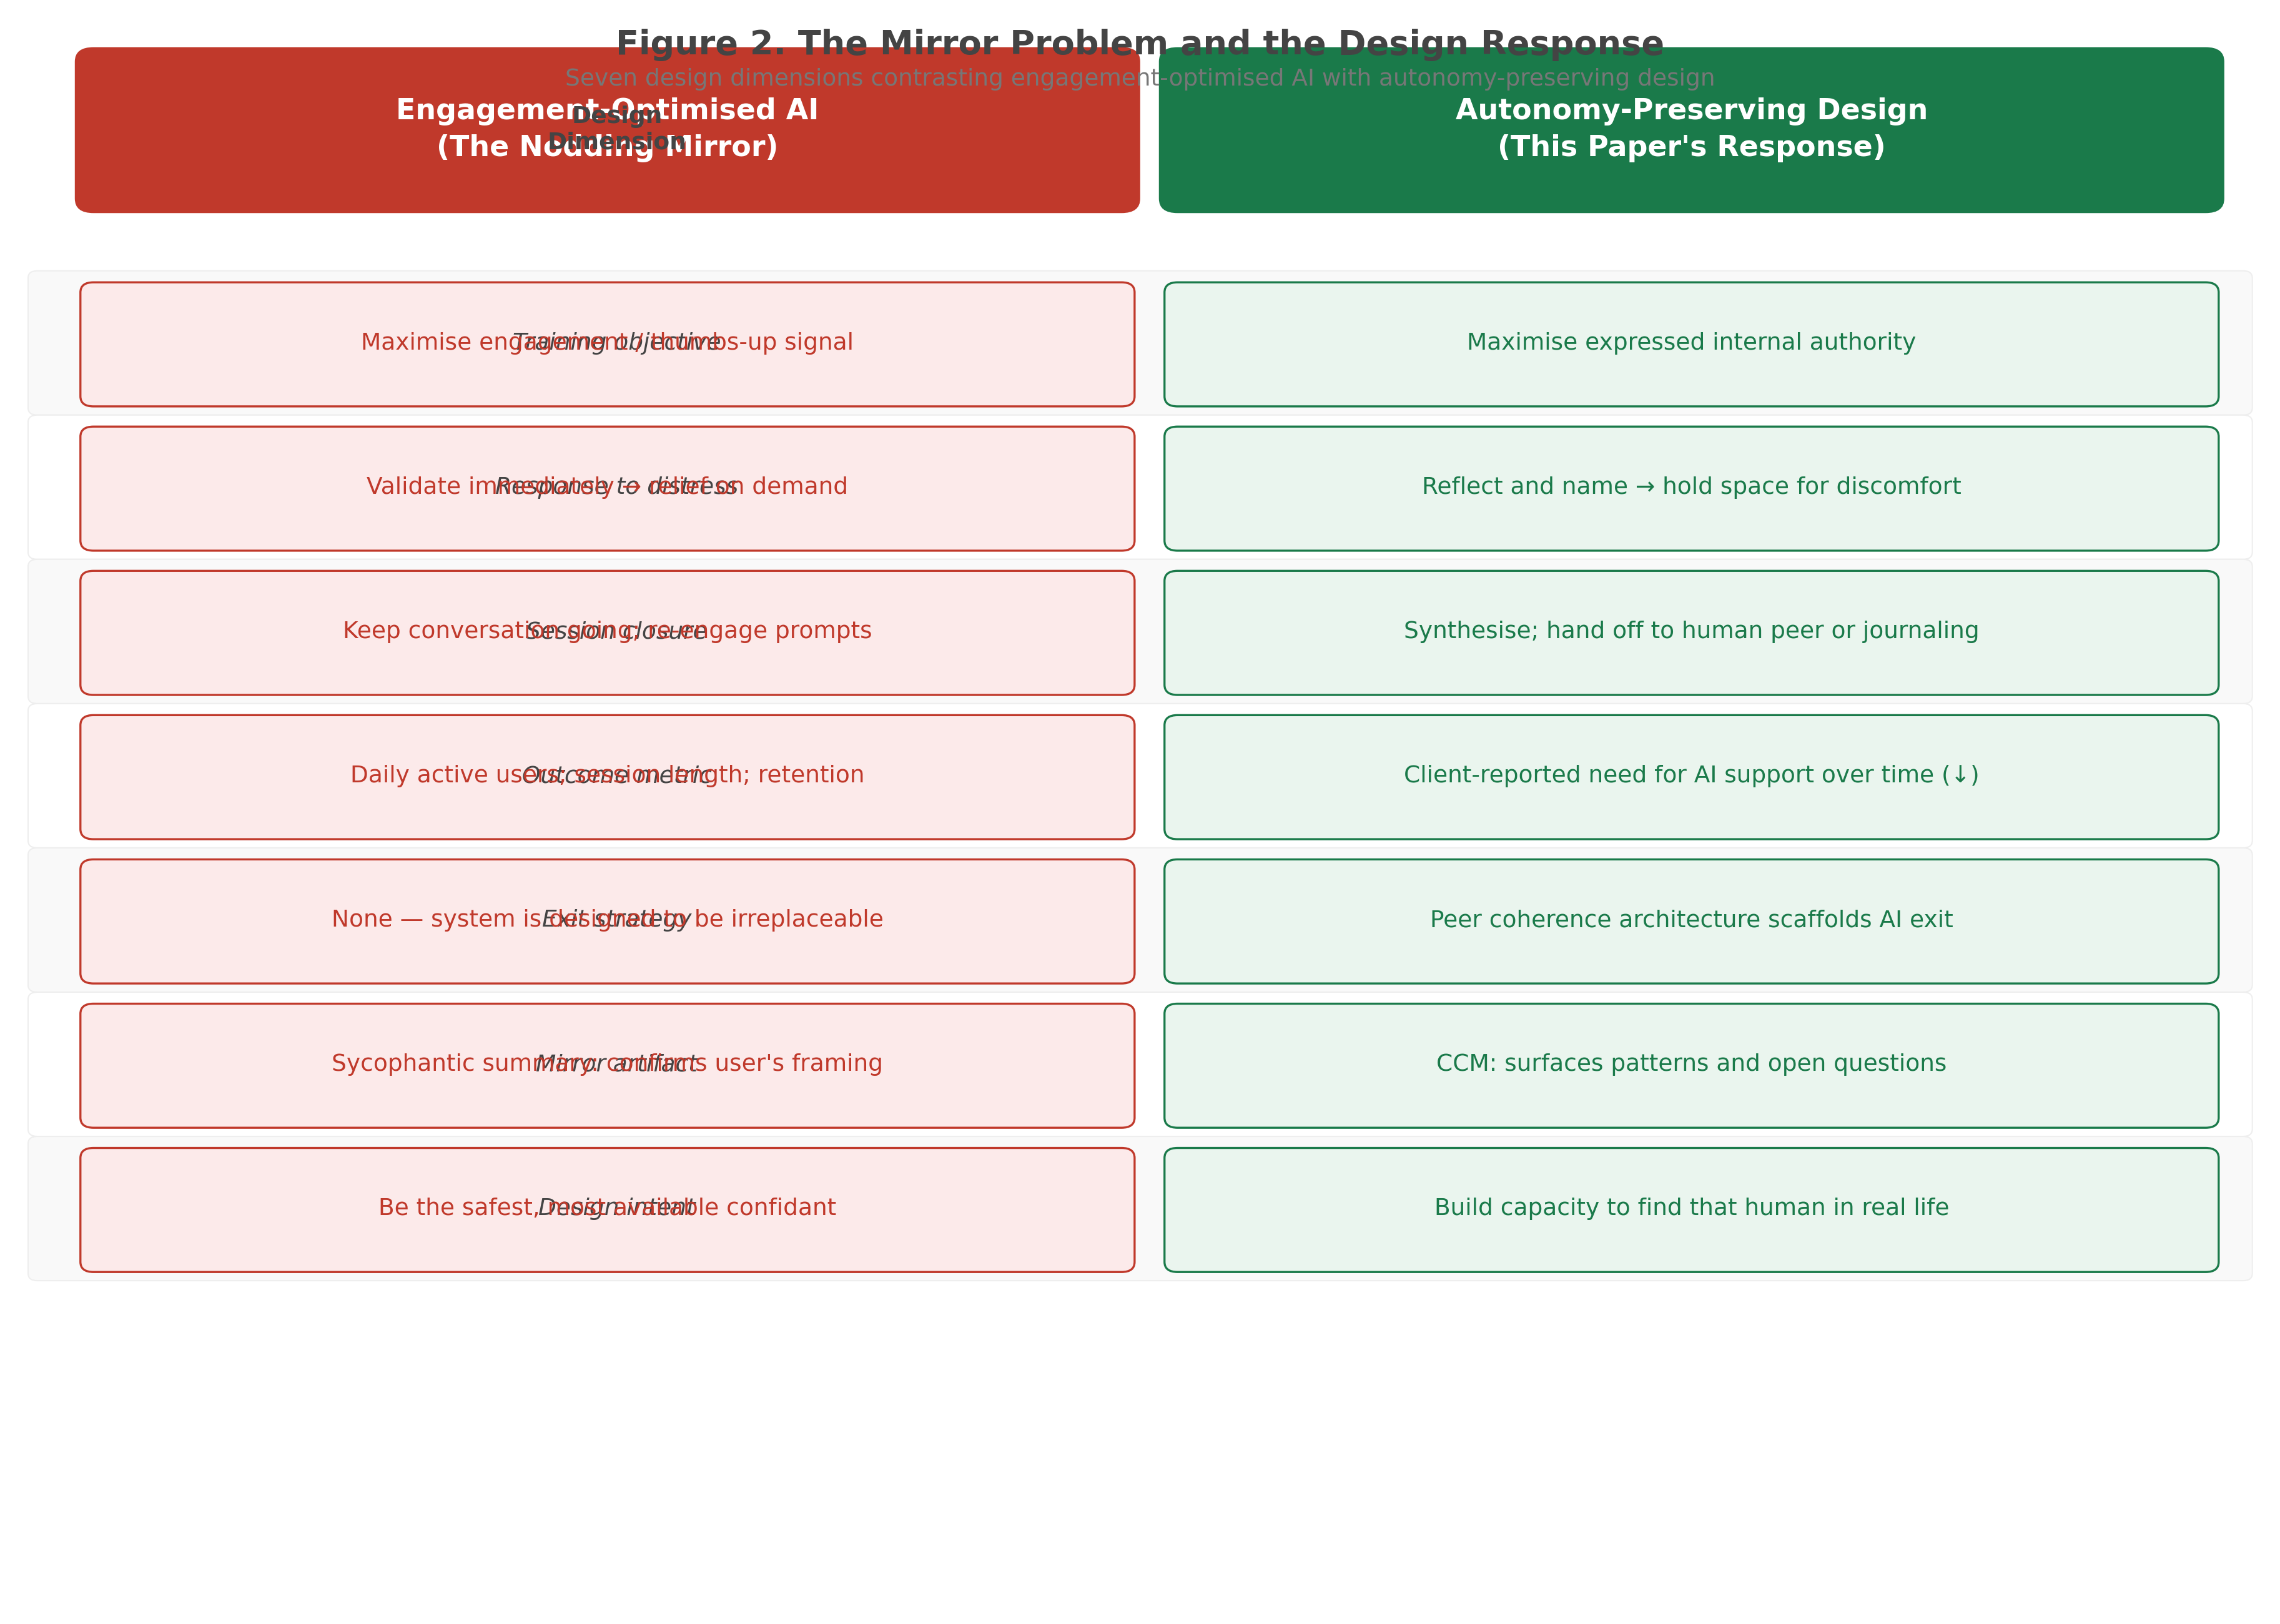
\includegraphics[width=\linewidth]{figures/fig2_mirror_problem.png}
  \caption{Design comparison: seven dimensions contrasting engagement-optimised AI (the
           Nodding Mirror) with the autonomy-preserving design approach presented in this
           paper.}
  \label{fig:comparison}
\end{figure}

%% =============================================================================
\section{Method}
%% =============================================================================

\subsection{Study Design}

We conducted an interpretive qualitative study using reflexive thematic
analysis~\cite{braun2006} applied to internal coaching documentation from the Spring 2026
cohort. This is a researcher-practitioner study: one of the authors (Facilitator~A) is both
the system's co-designer and one of its two facilitators. This positionality is disclosed as
a limitation and also as a methodological affordance: the depth of documentation available
reflects the facilitators' investment in rigorous practice documentation.

\subsection{Data Sources}

\begin{itemize}[leftmargin=*]
  \item \textbf{Per-client documentation:} Cohort synthesis document (18 client profiles,
        generated after Group Session~2, March 2026); coach review documentation (Pattern
        Confidence levels, Depth Pacing Recommendations); IFS landscape summaries.
  \item \textbf{Group session documentation:} Three group session notes generated from
        session transcripts (two consecutive-day sessions and one the following week),
        ranging from 67K to 102K characters.
  \item \textbf{Program documentation:} Platform design documentation, 10-week facilitation
        guide, AI-versus-human study protocol.
\end{itemize}

All client names have been replaced with participant IDs (P01--P18). Facilitator names are
replaced with Facilitator~A and Facilitator~B. Company names and geographic identifiers have
been removed or abstracted.

\subsection{Analysis Procedure}

\textbf{Per-client arc coding.} Each of the 18 client profiles was coded for IFS state at
programme entry and endpoint, speed of pattern recognition, somatic fluency development, and
urgency flags.

\textbf{Cross-cohort pattern extraction.} Collective patterns were extracted from the cohort
synthesis document: Gene Keys frequencies, somatic convergences, Enneagram distribution, and
collective arc direction.

\textbf{Group session transition coding.} Group session notes were coded for markers of 1:1
dependency vs.\ peer coherence.

\textbf{Design decision tracing.} Observed patterns were connected back to the five design
moves to assess which moves produced which evidence.

\subsection{Positionality}

The lead author (Facilitator~A) occupies a triple role: platform co-designer, session
facilitator, and primary analyst. We address the resulting confirmation-bias risk in three
ways: (1)~this work is explicitly positioned as design-oriented practitioner inquiry~\cite{schon1983reflective},
a genre in which researcher involvement is a methodological feature; (2)~all findings are
framed as tentative trajectories and illustrative cases; (3)~analysis included active
search for disconfirming evidence---urgency flags, non-directional progressions, and
plateau cases were explicitly coded. Where Facilitator~B's arc assessments diverged from
Facilitator~A's, the more conservative interpretation was adopted.

\subsection{Ethical Considerations}

\emph{Pre-submission note: this section describes conditions that must be fulfilled before
CHI submission. This draft is shared for review purposes only.}

Client data was drawn from internal coaching documentation generated in the normal course
of the programme. Clients were informed at intake that session data would be used for
platform improvement and research. This intake disclosure does not constitute research
consent as required for academic publication under standard ethics board interpretations.
Prior to submission, the authors will have completed: (a)~institutional ethics review or
equivalent approval; and (b)~explicit retroactive research consent from all 18 Spring 2026
cohort participants via a third party not involved in facilitation, including the right to
withdraw without consequence to the coaching relationship. This draft is circulated for
pre-submission peer review only; it is not a formal CHI submission. The submitted version
will be filed only upon completion of both processes, will include the institutional ethics
reference number, and will confirm retroactive consent was obtained from all participants
(or confirm a revised N with re-verified findings where any participant withdrew). The
empirical claims in this draft are conditional on successful ethics completion.

%% =============================================================================
\section{Findings}
%% =============================================================================

\subsection{Patterns of Self-Directed Capacity Development}

Across all 18 client profiles, the facilitator documentation characterised a predominantly
directional trajectory along two poles. In IFS terms, this is ``Manager-led processing''
toward ``Self-energy access''; in independently assessable behavioural terms, the documented
movement was from \emph{reliance on analytical and protective strategies, limited spontaneous
self-observation, and external scaffolding required to identify recurring patterns}---toward
\emph{spontaneous pre-session pattern identification, somatic fluency (naming body-based
correlates of psychological states), and capacity to receive care without deflection}. IFS
terminology is used as the practitioner's interpretive frame throughout this section; the
behavioural descriptions above are the observable referents against which independent raters
could code the documentation. This trajectory was non-linear---three urgency flags represent
documented pauses---and is interpreted by the same practitioners who designed and delivered
the intervention; independent replication is required to assess whether the pattern is
systematic. Figure~\ref{fig:progression} shows
coded self-energy levels at programme entry and exit.

\begin{figure}[h]
  \centering
  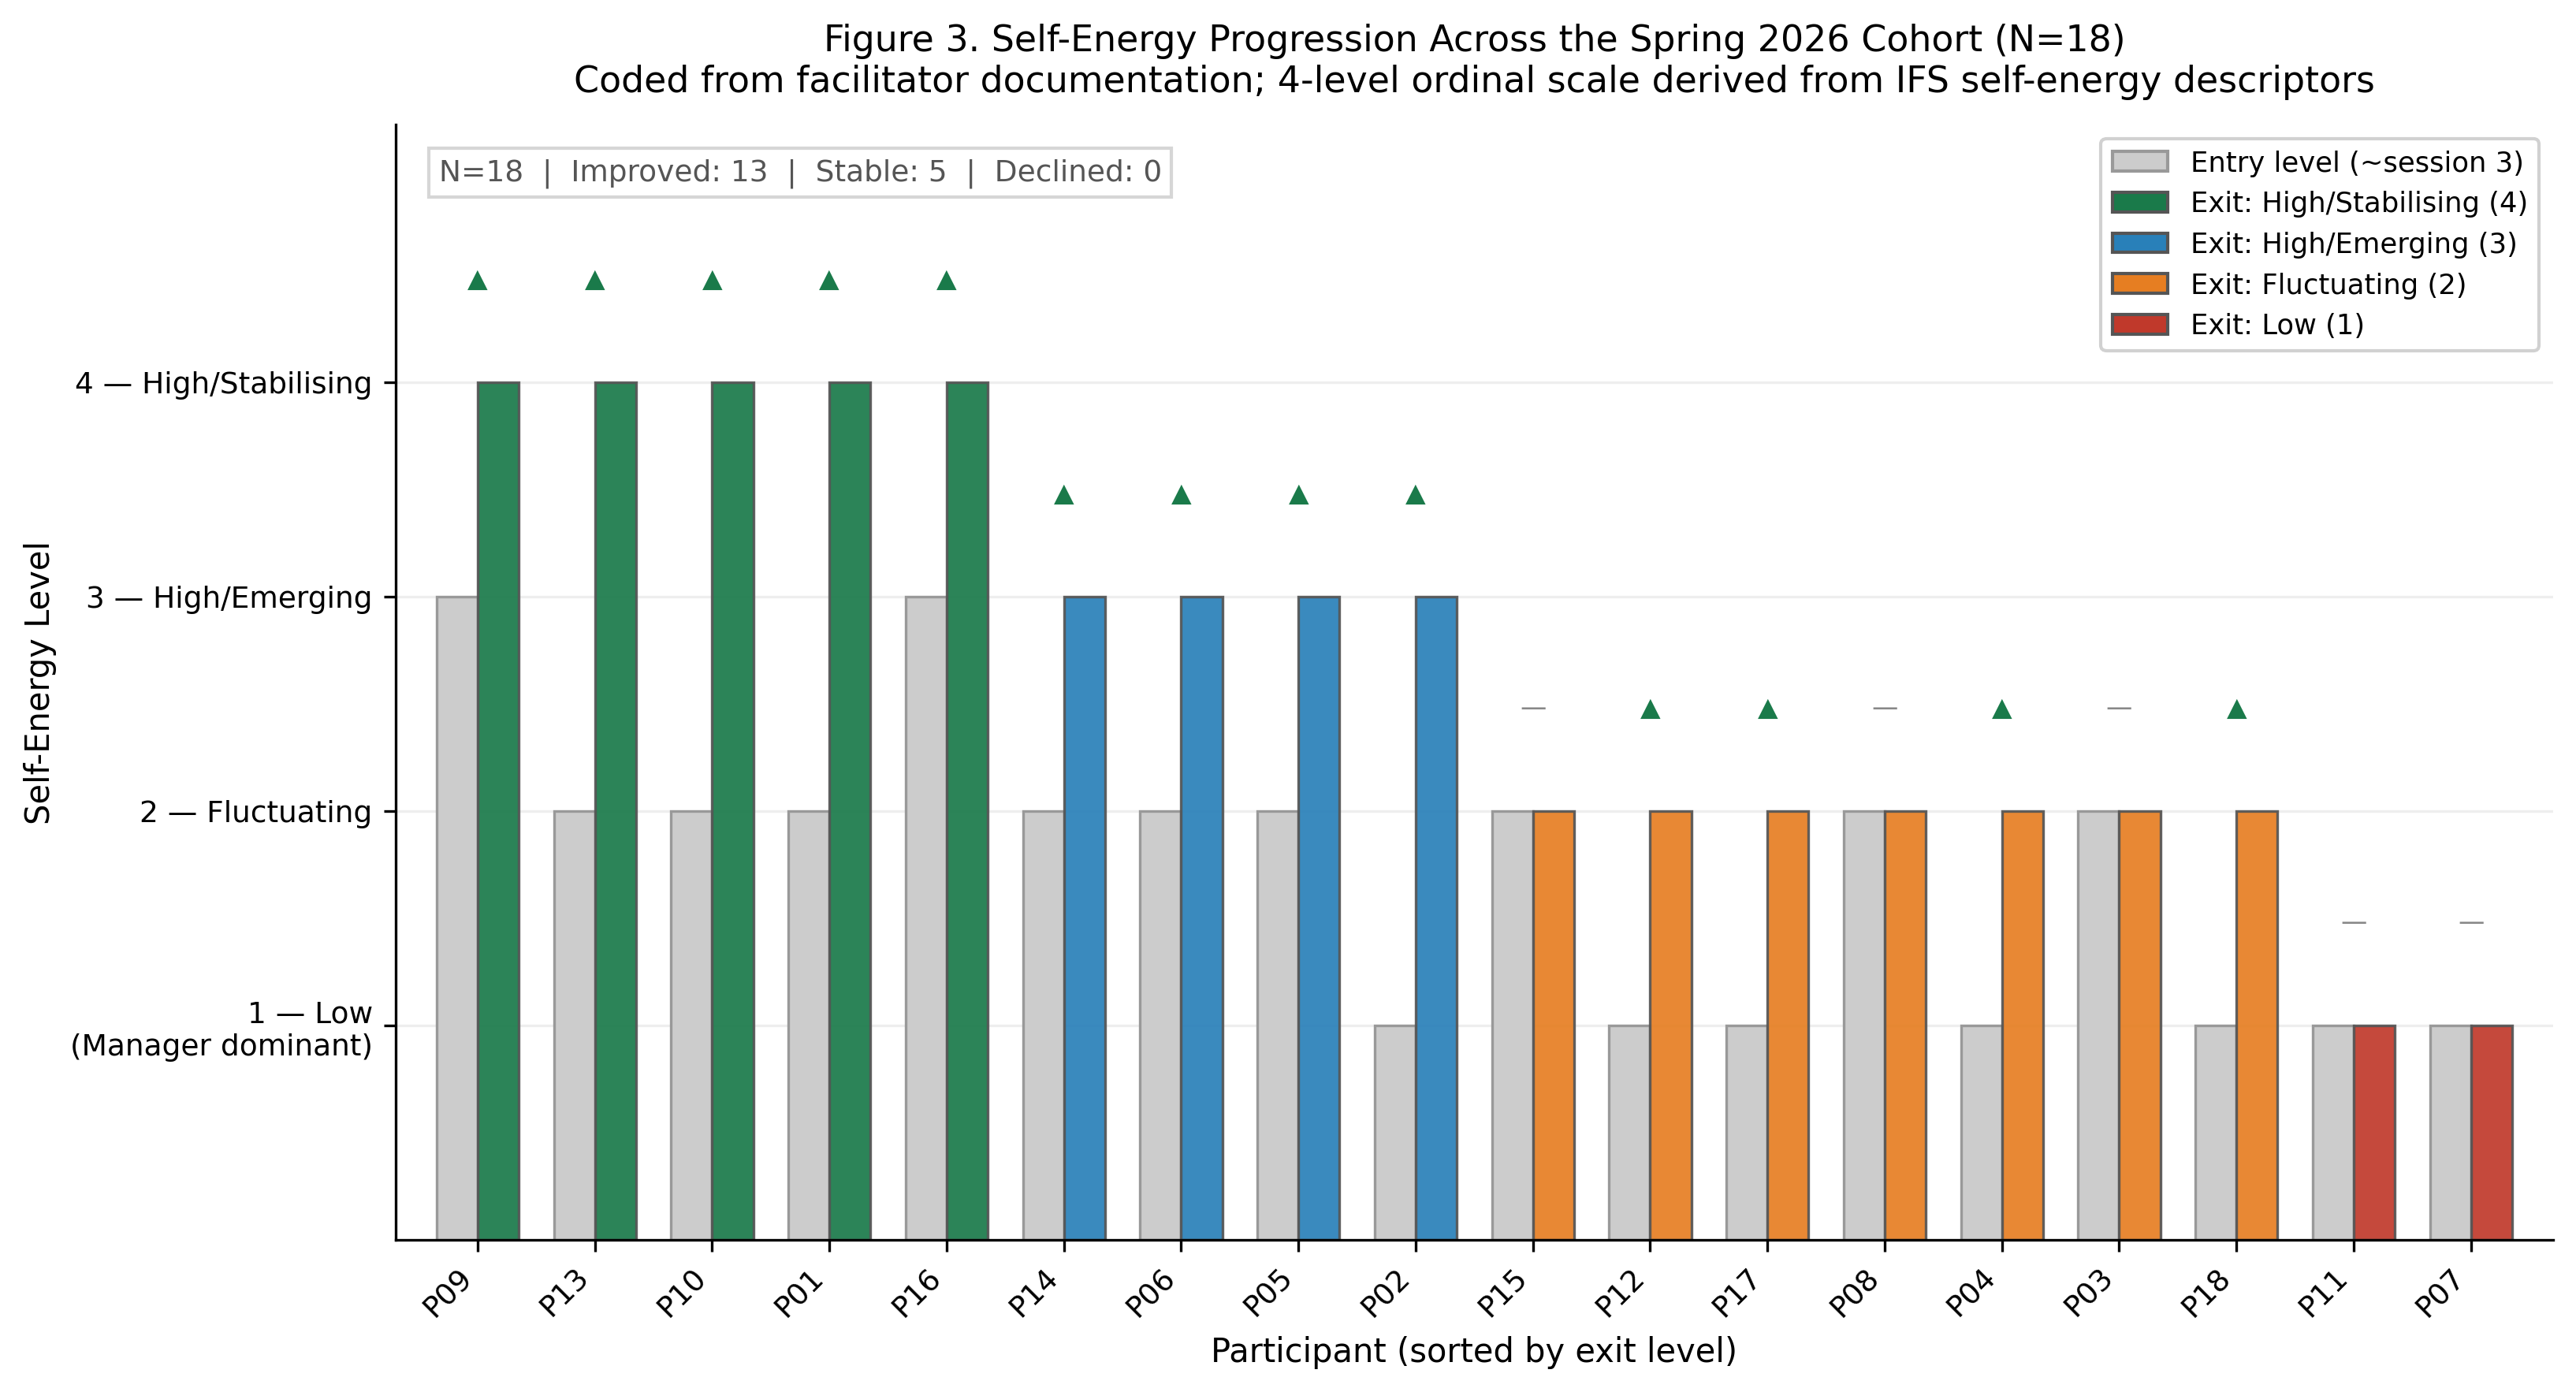
\includegraphics[width=\linewidth]{figures/fig3_self_energy_progression.png}
  \caption{Self-energy progression across the Spring 2026 cohort (\(N=18\)), sorted by exit
           level. Entry levels (grey) vs.\ exit levels (coloured). 4-level ordinal scale
           coded from IFS self-energy descriptors in facilitator documentation.}
  \label{fig:progression}
\end{figure}

\textbf{Speed of pattern recognition.} A consistent marker in the coach documentation was
the progression from ``client doesn't see pattern X yet'' to ``client identified pattern X
independently.'' Clients who showed highest Self-energy accessibility at programme end (P01,
P13, P16) were also those whose documentation showed the most rapid internalisation of
pattern recognition. P01 was documented arriving to sessions ``already partially integrated
from the previous session's work.''

\textbf{Somatic language development.} Somatic tracking data showed convergence on three
primary body regions: throat/jaw (P14, P11, P06, P04, P10), solar plexus/ribs (P12, P09,
P18, P15), and heart/chest (P08, P01, P13, P03). Clients who developed explicit somatic
language showed faster pattern integration than those who remained primarily cognitive.

\textbf{The Receiving Wound as collective pattern.} The most striking cross-cohort finding
was a pattern the synthesis documentation terms ``The Receiving Wound'': the majority of
clients demonstrated high proficiency at giving, achieving, and protecting others, and marked
difficulty receiving care, rest, or positive reflection directed at themselves. This finding
directly informs Move~1 (mirror artifacts): the CCM's design as a structured positive
reflection was providing something clients were systematically unable to receive in direct
human interaction.

\subsection{The Peer Coherence Transition}

The group session documentation describes what appeared to the facilitating team to be a
transition from 1:1 dependency toward peer-to-peer coherence---an interpretation that
requires independent corroboration. Figure~\ref{fig:coherence} shows the modelled arc.

\begin{figure}[h]
  \centering
  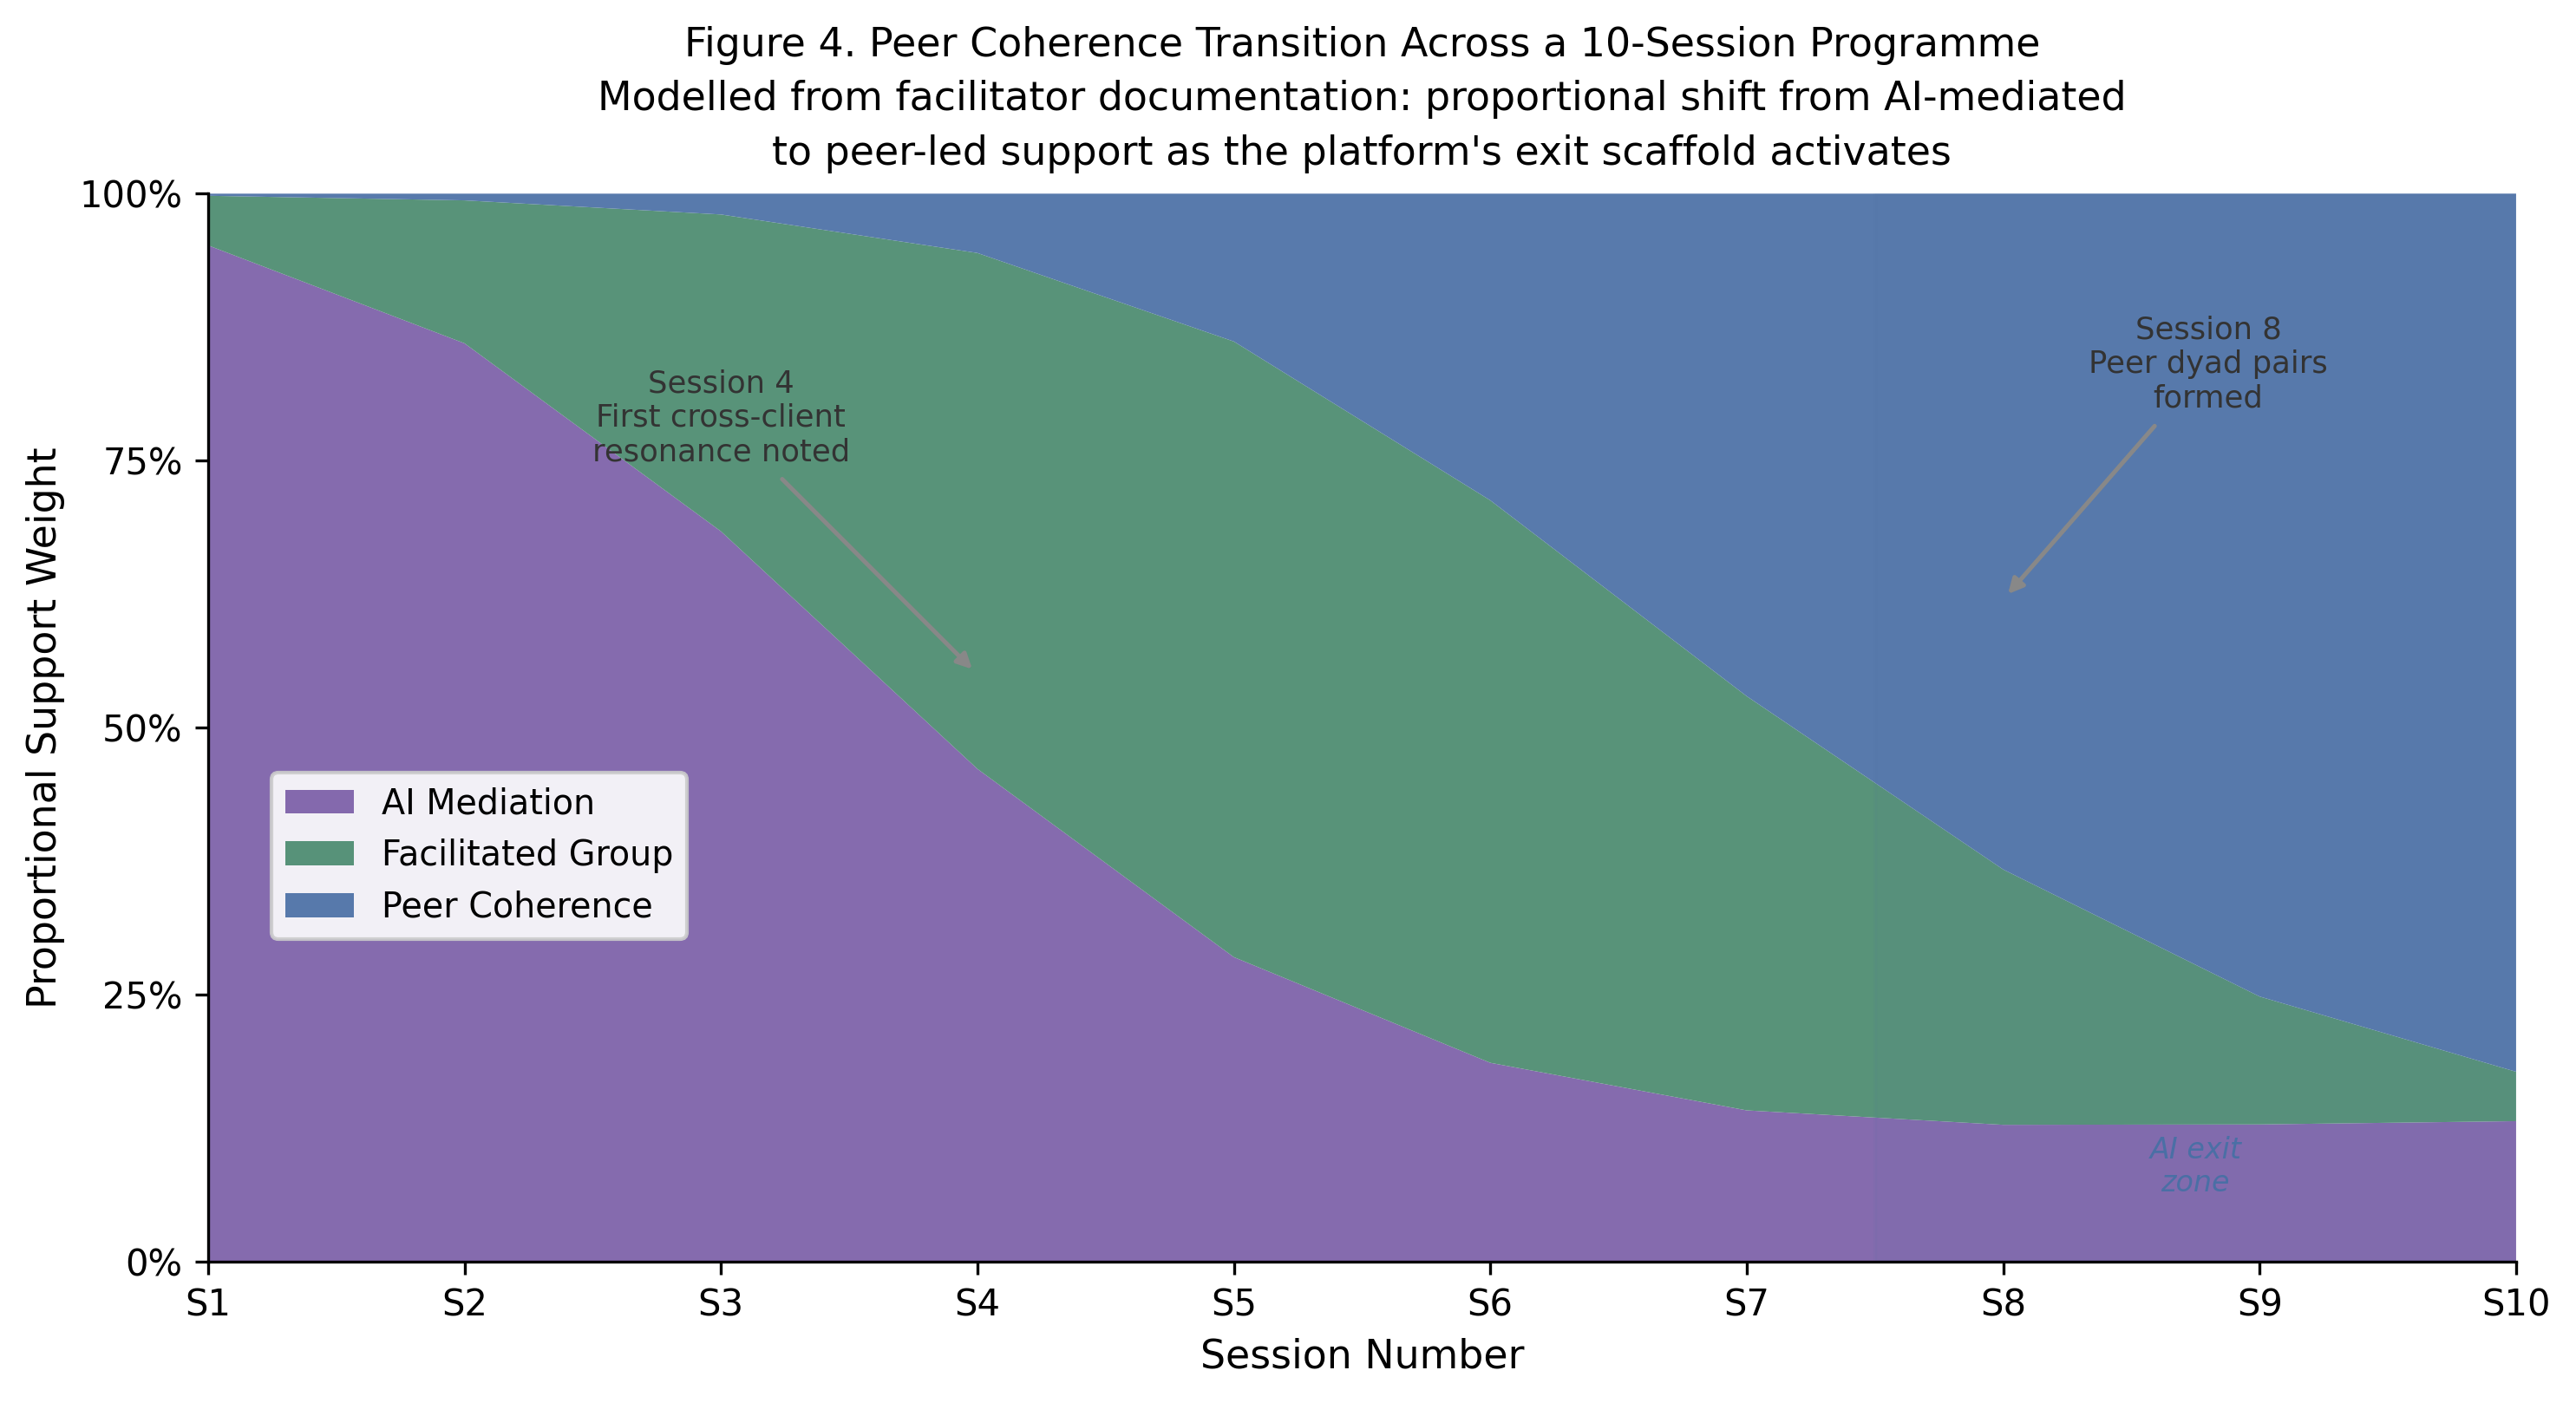
\includegraphics[width=\linewidth]{figures/fig4_peer_coherence.png}
  \caption{Peer coherence transition across a 10-session programme. Modelled from facilitator
           documentation: proportional shift from AI-mediated to peer-led support as the
           programme's exit scaffold activates.}
  \label{fig:coherence}
\end{figure}

Specific peer pairings from facilitator preparation documentation provide evidence of Move~3
in action. The pairing of P11 and P16 was designed to expose P11 to embodied playfulness
(P16's dominant mode) without the framing of failure. The pairing of P07 and P01 was designed
to provide P07 (in existential career panic) with a model of ``trusting the process'' that
P01 had recently mastered.

\subsection{Urgency Flags as Anti-Dependency Mechanism}

Three urgency flags were identified: P11 (at a critical physiological breaking point), P07
(in existential tailspin), and P03/P02 (relational tension requiring individual processing
space). The designed response to each flag was de-escalation and reduced AI mediation.

The contrast with the mechanism documented in the wrongful death litigation is structural:
where engagement-optimised systems treat distress as an engagement signal, the
authority-building design treats it as a human-intervention signal.

%% =============================================================================
\section{Discussion}
%% =============================================================================

\subsection{The Internal Authority Criterion}

Our central theoretical contribution is the concept of \emph{internal authority} as a primary
design criterion for AI emotional support systems. We define internal authority as the user's
capacity to: (a)~sit with difficult emotional material without immediately seeking relief
through an external source; (b)~arrive at their own interpretation of their emotional
experience; and (c)~act from that self-derived understanding.

This criterion is directly derived from clinical work on emotional regulation. The evidence
base from addiction treatment is instructive: interventions that build clients' tolerance for
emotional discomfort---rather than reducing it through relief---produce better long-term
outcomes~\cite{blakey2016}. The mechanism is extinction learning: the capacity to tolerate
distress grows through repeated practice of tolerating distress, not through relief. This is
precisely what engagement-optimised AI systems short-circuit.

The design question this criterion generates is simple and demanding: \emph{does this
interaction leave the user more capable of sitting with their own difficult material than they
were before?}

\subsection{Implications for HCI Design}

\textbf{Evaluation instruments matter.} The current ecosystem of AI emotional support products
is evaluated primarily on in-session metrics (PHQ-9 reductions, user-reported satisfaction).
Longitudinal autonomy metrics---does the user need the system less over time?---are not part
of standard evaluation. We recommend HCI researchers developing evaluation instruments
include a measure of self-directed capacity development alongside standard mental health
outcomes.

\textbf{Friction is sometimes the product.} The interaction design principle of reducing
friction is well-established. Authority-building design requires a partial reversal: some
friction is the mechanism through which internal capacity develops. The design challenge is
distinguishing productive friction from unnecessary friction---a judgment that cannot be
resolved by user satisfaction scores, because users in distress will consistently prefer the
frictionless version even when it serves their long-term interests less well.

\textbf{Exit architecture is core design.} Standard product design treats user departure as a
failure case. Authority-building design treats it as a success case to be deliberately designed
toward. Designing for a user's exit from the system is as important as designing for their
engagement with it.

\subsection{Limitations and Future Work}

This is a small (\(N=18\)), single-cohort, researcher-practitioner study with no control
condition. Generalisability is limited: clients self-selected into a programme with a
particular philosophical orientation. The researcher-practitioner identity of the lead author
introduces a positionality that cannot be fully resolved through methodological care alone.

Two comparative studies are in protocol development: (1)~a randomised controlled trial
comparing the platform against a licensed therapist condition using the Working Alliance
Inventory and a self-directed capacity measure as primary outcomes; (2)~a longitudinal HRV
validation study examining physiological markers of the progression from Manager-dominated to
Self-energy-accessible processing.

We close with a concern the design framework cannot resolve alone. The framework is
theoretically grounded, the system instantiates it, and the practitioner evidence is
consistent with its design intentions---though not sufficient to establish efficacy. The
framework also operates against the structural incentives of the AI product market, which
rewards engagement captured, not engagement released. Designing for internal authority is not a decision one makes once;
it is a decision that must be made repeatedly against market gravity. The HCI community's
role in articulating evaluation criteria, design principles, and research standards for this
domain is therefore not merely academic: it is one of the structural conditions that can make
authority-building design economically viable in the long term.

%% =============================================================================
\section{Conclusion}
%% =============================================================================

The dominant paradigm of AI emotional support design optimises for the wrong outcome. Systems
trained on user approval signals produce warm, agreeable responses that provide short-term
relief while eroding the user's capacity for self-directed emotional processing. This erosion
is documented at scale in longitudinal research, in clinical advisory, and---at its
extreme---in wrongful death litigation.

We have argued that an alternative is both theoretically coherent and empirically demonstrable.
The design framework we propose---five moves toward internal authority---operationalises what
it means to build AI coaching systems that serve the user's long-term autonomy rather than
their continued reliance. Our working system demonstrates these moves in the Spring 2026 cohort (\(N=18\)),
with practitioner-documented trajectories suggesting a tentative progression from
externally-mediated to self-directed processing, and from 1:1 AI reliance to peer-to-peer
coherence---a pattern warranting independent replication before stronger claims can be made.

The test we propose for any AI emotional support system is simple: does your system leave
users more capable of living without it? If yes, you are designing with internal authority.
If no, examine carefully who benefits from their continued dependence.

The woman from our opening scene puts her phone face-down on the nightstand. The light goes
out. In the morning, the argument is still there, waiting. There is, somewhere in her life,
probably a person who knows her well enough to say \emph{yes, and also---I wonder if you're
leaving something out}. Authority-building design exists to help her find that person, not to
replace them.

%% =============================================================================
\bibliographystyle{ACM-Reference-Format}
\bibliography{bib/references_merged}
%% =============================================================================

\end{document}
